% !TEX TS-program = lualatex
% !TEX encoding = UTF-8 Unicode		

\documentclass[11pt, letterpaper]{article}

%%BIBLIOGRAPHY- This uses biber/biblatex to generate bibliographies according to the 
%%Unified Style Sheet for Linguistics
\usepackage[main=american, german]{babel}% Recommended
\usepackage{csquotes}% Recommended
\usepackage[backend=biber,
		style=unified,
		maxcitenames=3,
		maxbibnames=99,
		natbib,
		url=false]{biblatex}
\addbibresource{../Library.bib}
\setcounter{biburlnumpenalty}{100}  % allow URL breaks at numbers
%\setcounter{biburlucpenalty}{100}   % allow URL breaks at uppercase letters
%\setcounter{biburllcpenalty}{100}   % allow URL breaks at lowercase letters

%%TYPOLOGY
\usepackage[svgnames]{xcolor} % Specify colors by their 'svgnames', for a full list of all colors available see here: http://www.latextemplates.com/svgnames-colors
%\usepackage[compact]{titlesec}
%\titleformat{\section}[runin]{\normalfont\bfseries}{\thesection.}{.5em}{}[.]
%\titleformat{\subsection}[runin]{\normalfont\scshape}{\thesubsection}{.5em}{}[.]
\usepackage[hmargin=.5in,vmargin=.5in]{geometry}  %Margins          
\usepackage{graphicx}	%Inserting graphics, pictures, images 		
\usepackage{stackengine} %Package to allow text above or below other text, Also helpful for HG weights 
\usepackage{fontspec} %Selection of fonts must be ran in XeLaTeX
\usepackage{amssymb} %Math symbols
\usepackage{amsmath} % Mathematical enhancements for LaTeX
\usepackage{setspace} %Linespacing
\usepackage{multicol} %Multicolumn text
\usepackage{enumitem} %Allows for continuous numbering of lists over examples, etc.
\usepackage{multirow} %Useful for combining cells in tablesbrew 
\usepackage{hanging}
\usepackage{fancyhdr} %Allows for the 
\pagestyle{fancy}
\fancyhead[L]{\textit{TITLE}} 
\fancyhead[R]{\textit{\today}} 
\fancyfoot[L,R]{} 
\fancyfoot[C]{\thepage} 
\renewcommand{\headrulewidth}{0.4pt}
\setlength{\headheight}{14.5pt} % ...at least 14.49998pt
% \usepackage{fourier} % This allows for the use of certain wingdings like bombs, frowns, etc.
% \usepackage{fourier-orns} %More useful symbols like bombs and jolly-roger, mostly for OT
\usepackage[colorlinks,allcolors={black},urlcolor={blue}]{hyperref} %allows for hyperlinks and pdf bookmarks
% \usepackage{url} %allows for urls
% \def\UrlBreaks{\do\/\do-} %allows for urls to be broken up
\usepackage[normalem]{ulem} %strike out text. Handy for syntax
\usepackage{tcolorbox}
\usepackage{datetime2}
\usepackage{caption}
\usepackage{subcaption}

%%FONTS
\setmainfont{Libertinus Serif}
\setsansfont{Libertinus Sans}
\setmonofont[Scale=MatchLowercase]{Libertinus Mono}

%%PACKAGES FOR LINGUISTICS
%\usepackage{OTtablx} %Generating tableaux with using TIPA
% \usepackage[noipa]{OTtablx} % Use this one generating tableaux without using TIPA
%\usepackage[notipa]{ot-tableau} % Another tableau drawing packing use for posters.
% \usepackage{linguex} % Linguistic examples
% \usepackage{langsci-linguex} % Linguistic examples
\usepackage{langsci-gb4e} % Language Science Press' modification of gb4e
% \usepackage{langsci-avm} % Language Science Press' AVM package
\usepackage{tikz} % Drawing Hasse diagrams
% \usepackage{pst-asr} % Drawing autosegmental features
\usepackage{pstricks} % required for pst-asr, OTtablx, pst-jtree.
% \usepackage{pst-jtree} 	% Syntax tree draawing software
% \usepackage{tikz-qtree}	% Another syntax tree drawing software. Uses bracket notation.
\usepackage[linguistics]{forest}	% Another syntax tree drawing software. Uses bracket notation.
% \usepackage{ling-macros} % Various linguistic macros. Does not work with linguex.
% \usepackage{covington} % Another linguistic examples package.
\usepackage{leipzig} %	Offers support for Leipzig Glossing Rules

%%LEIPZIG GLOSSING FOR ZAPOTEC
\newleipzig{el}{el}{elder}	% Elder pronouns
\newleipzig{hu}{hu}{human}	% Human pronouns
\newleipzig{an}{an}{animate}	% Animate pronouns
\newleipzig{in}{in}{inanimate}	% Inanimate pronouns
\newleipzig{pot}{pot}{potential}	% Potential Aspect
\newleipzig{cont}{cont}{continuative}	% Continuative Aspect
% \newleipzig{pot}{pot}{potential}	% Potential Aspect
\newleipzig{stat}{stat}{stative}	% Potential Aspect
\newleipzig{and}{and}{andative}	% Andative Aspect
\newleipzig{ven}{ven}{venative}	% Venative Aspect
% \newleipzig{res}{res}{restitutive}	% Restitutive Aspect
\newleipzig{rep}{rep}{repetitive}	% Repetitive Aspect

%%TITLE INFORMATION
% \title{TITLE}
% \author{Mykel Loren Brinkerhoff}
% \date{\today}

%%MACROS
\newcommand{\sub}[1]{\textsubscript{#1}}
\newcommand{\supr}[1]{\textsuperscript{#1}}

\makeatletter
\renewcommand{\paragraph}{%
  \@startsection{paragraph}{4}%
  {\z@}{0ex \@plus 1ex \@minus .2ex}{-1em}%
  {\normalfont\normalsize\bfseries}%
}
\makeatother
\parindent=10pt


\begin{document}
	
%%If using linguex, need the following commands to get correct LSA style spacing
%% these have to be after  \begin{document}
	% \setlength{\Extopsep}{6pt}
	% \setlength{\Exlabelsep}{9pt}		%effect of 0.4in indent from left text edge

	
%% Line spacing setting. Comment out the line spacing you do not need. Comment out all if you want single spacing.
%	\doublespacing
%	\onehalfspacing
	
\begin{center}
	\textbf{Testing the Laryngeal Complexity Hypothesis: Evidence from Santiago Laxopa Zapotec}
\end{center}
%\maketitle
%\maketitleinst
% \thispagestyle{fancy}
\thispagestyle{empty}

\paragraph{Introduction:}
Most descriptions about the interaction between tone and phonation are based on South East and East Asian languages \citep[e.g.,][]{masicaDefiningLinguisticArea1976,thurgoodVietnameseTonogenesisRevising2002,michaudComplexTonesEast2012,brunelleTonePhonationSoutheast2016,kuangCovariationVoiceQuality2017}.
These descriptions have lead to widespread claims about what is possible in languages with tone and phonation, specifically that tone and phonation are co-dependent. 
This means that certain tones will bear specific phonations or that certain phonation types only appear with certain tones. 
For example, Mandarin's tone 3 is associated with creaky voice \citep{hockettPeipingPhonology1947} and Vietnamese's low falling tone is associated with breathy voice \citep{thurgoodVietnameseTonogenesisRevising2002}.
This, however, is not the true for Oto-Manguean languages where tone and phonation are independent from one another \citep{silvermanLaryngealComplexityOtomanguean1997}.

\paragraph{The Laryngeal Complexity Hypothesis:} Despite being independent from one another, tone and phonation need to interact in a way that is perceptually salient. This need for perceptual saliency led to the proposing of the \textsc{Laryngeal Complexity Hypothesis} \citep[LCH;][]{silvermanLaryngealComplexityOtomanguean1997,blankenshipTimeCourseBreathiness1997,blankenshipTimingNonmodalPhonation2002}. The LHC's basic premise is that for tone and phonation to be best perceived there needs to be an ordering or phasing between the gestures for tone and phonation. If there was no strict ordering of the gestures for tone and phonation then the cues for tone and/or phonation will have interference, see Figure~\ref{fig:GlottalGestures} for a graphical illustration. \posscitet{dicanioCoarticulationToneGlottal2012} study exploring the LCH in Itunyoso Trique found exactly this interference. \citeauthor{dicanioCoarticulationToneGlottal2012} showed that when there is a large overlap between the gestures for tone and phonation that the f0 signal is perturbed by the glottal gestures for phonation. 

This paper investigates the LCH's role in Santiago Laxopa Zapotec (SLZ), an understudied Oto-Manguean language spoken by approximately 1000 people in the municipality of Santiago Laxopa in the Sierra Norte of Oaxaca, Mexico. 

\paragraph{Description of SLZ tone and phonation:} 
SLZ, like other Oto-Manguean languages, contains a robust systems of both tone and phonation which are independent from each other. SLZ has five surface tonal patterns on syllables: three level tones H(igh), M(id), L(ow) and two contour tones HL and MH. Vowels in SLZ, additionally have four phonations types: Modal, Breathy, Checked, and Laryngealized. 
These different tones and voice qualities are allowed to appear essentially independent from one other in the nominal domain with the only exceptions being H with breathy phonation and MH with checked tone.

\paragraph{Methodology:} 
Data was collected from 18 native SLZ consultants living in Santa Cruz, CA in person and in Santiago Laxopa, Ixtlán, Oaxaca, Mexico (11 female).  
Consultants were recorded repeating three times the phrase \textit{shnia' WORD chone las.} `I say WORD three times' with each of the 77 target words.
Vowels were extracted from the resulting audio files and spectral-tilt measurements were generated for each third of the vowel using VoiceSauce \citep{shueVOICESAUCEProgramVoice2009} following \citet{garellekAcousticConsequencesPhonation2011}. The results were then analyzed in R \citep{rcoreteamLanguageEnvironmentStatistical2021} using a mixed-effects linear regression with f0 as fixed variable and speaker and word being random variables to determine to what extent f0 is affected by phonation similar to \citet{dicanioCoarticulationToneGlottal2012}.  

\paragraph{Results:}
The spectral-tilt analysis shows that for both of the male and female speakers from California that H1-A3 is the best measurement for breathy phonation contrary to \posscitet{espositoVariationContrastivePhonation2010} observations that female speakers of Zapotec are best characterized by H1-H2. It is true that H1-H2 best characterized the checked and laryngealized vowels, both associated with creakiness, in the female. The male's phonation types were best represented by H1-A3 confirming \posscitet{espositoVariationContrastivePhonation2010}'s observation that male Zapotec speakers are best characterized by this spectral-tilt measurement. Box graphs showing the spectral-tilt measurement for the final third of the vowel for FSR (female) and RD (male) are presented in Figure~\ref{fig:h1h2third} for H1-H2 and Figure~\ref{fig:h1a3third} for H1-A3.

Preliminary results of the mixed-effects linear regression drawn from the two speakers living in California show that there was no effect of phonation on f0 in any portion of the vowel. However, further data is being collected in Santiago Laxopa to verify the results.

\paragraph{Upshot:}
This paper has provided a brief introduction to the tonal and phonation systems of Santiago Laxopa Zapotec, an understudied variety of Sierra Norte Zapotec. This system is important for studying the interaction of tone and phonation because of the complex interactions between tone and phonation that are found in this language. Because any phonation type can co-occur with any tone this presented a unique opportunity to see how the language compensates for using larynx for both tone and phonation. This paper has shown, by using language data elicitation data from SLZ, that the LCH \citep{silvermanLaryngealComplexityOtomanguean1997,blankenshipTimeCourseBreathiness1997, blankenshipTimingNonmodalPhonation2002} appears to be the best model of accounting for how tone and phonation interact. 



\newpage
\begin{center}
	\textbf{Figures and Tables}
\end{center}
\thispagestyle{empty}
\begin{figure}[!ht]
	\centering
	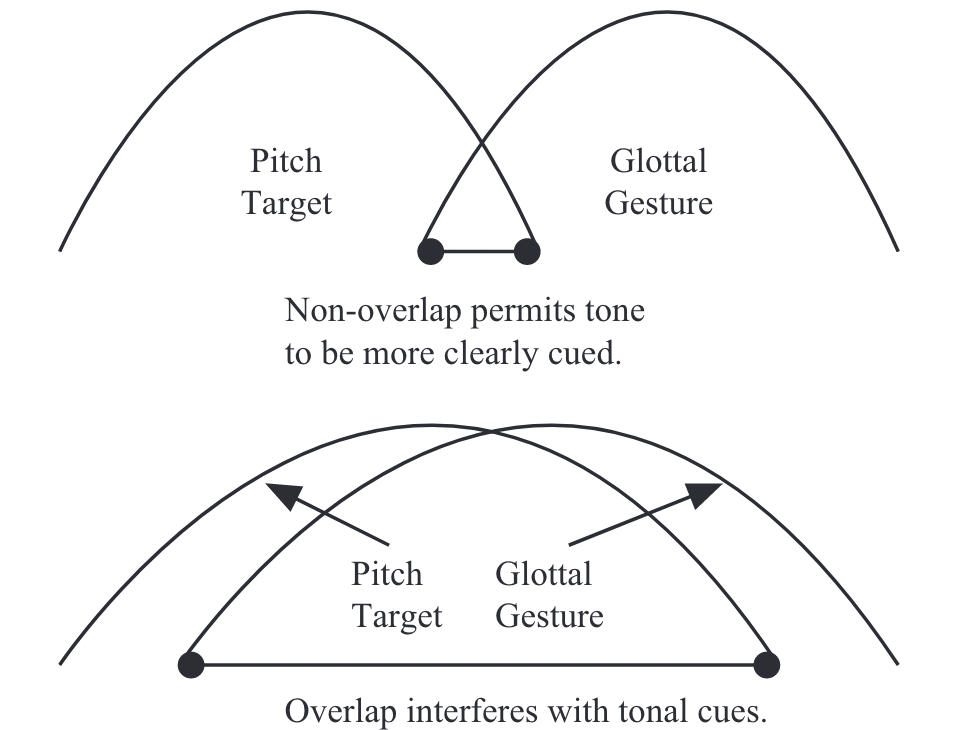
\includegraphics[width=.4\textwidth]{../Gestures.png}
	\caption{Representation taken from \citet{dicanioCoarticulationToneGlottal2012}.}
	\label{fig:GlottalGestures}
\end{figure}

\begin{figure}[!ht]
	\centering
	\begin{subfigure}{.5\textwidth}
		\centering
		\includegraphics[width=0.9\textwidth]{../mean_FSR_h1h2_3rd.png}
		\caption{FSR's H1-H2 values.}
		\label{fig:FSRh1h2third} 
	\end{subfigure}%
	\begin{subfigure}{.5\textwidth}
		\centering
		\includegraphics[width=0.9\textwidth]{../mean_RD_h1h2_3rd.png}
		\caption{RD's H1-H2 values.}
		\label{fig:RDh1h2third} 
	\end{subfigure}
	\caption{Mean H1-H2 values for the final third of the vowel according to each phonation type. }
	\label{fig:h1h2third}
\end{figure}

\begin{figure}[!ht]
	\centering
	\begin{subfigure}{.5\textwidth}
		\centering
		\includegraphics[width=0.9\textwidth]{../mean_FSR_h1a3_third.png}
		\caption{FSR's H1-A3 values.}
		\label{fig:FSRh1a3third} 
	\end{subfigure}%
	\begin{subfigure}{.5\textwidth}
		\centering
		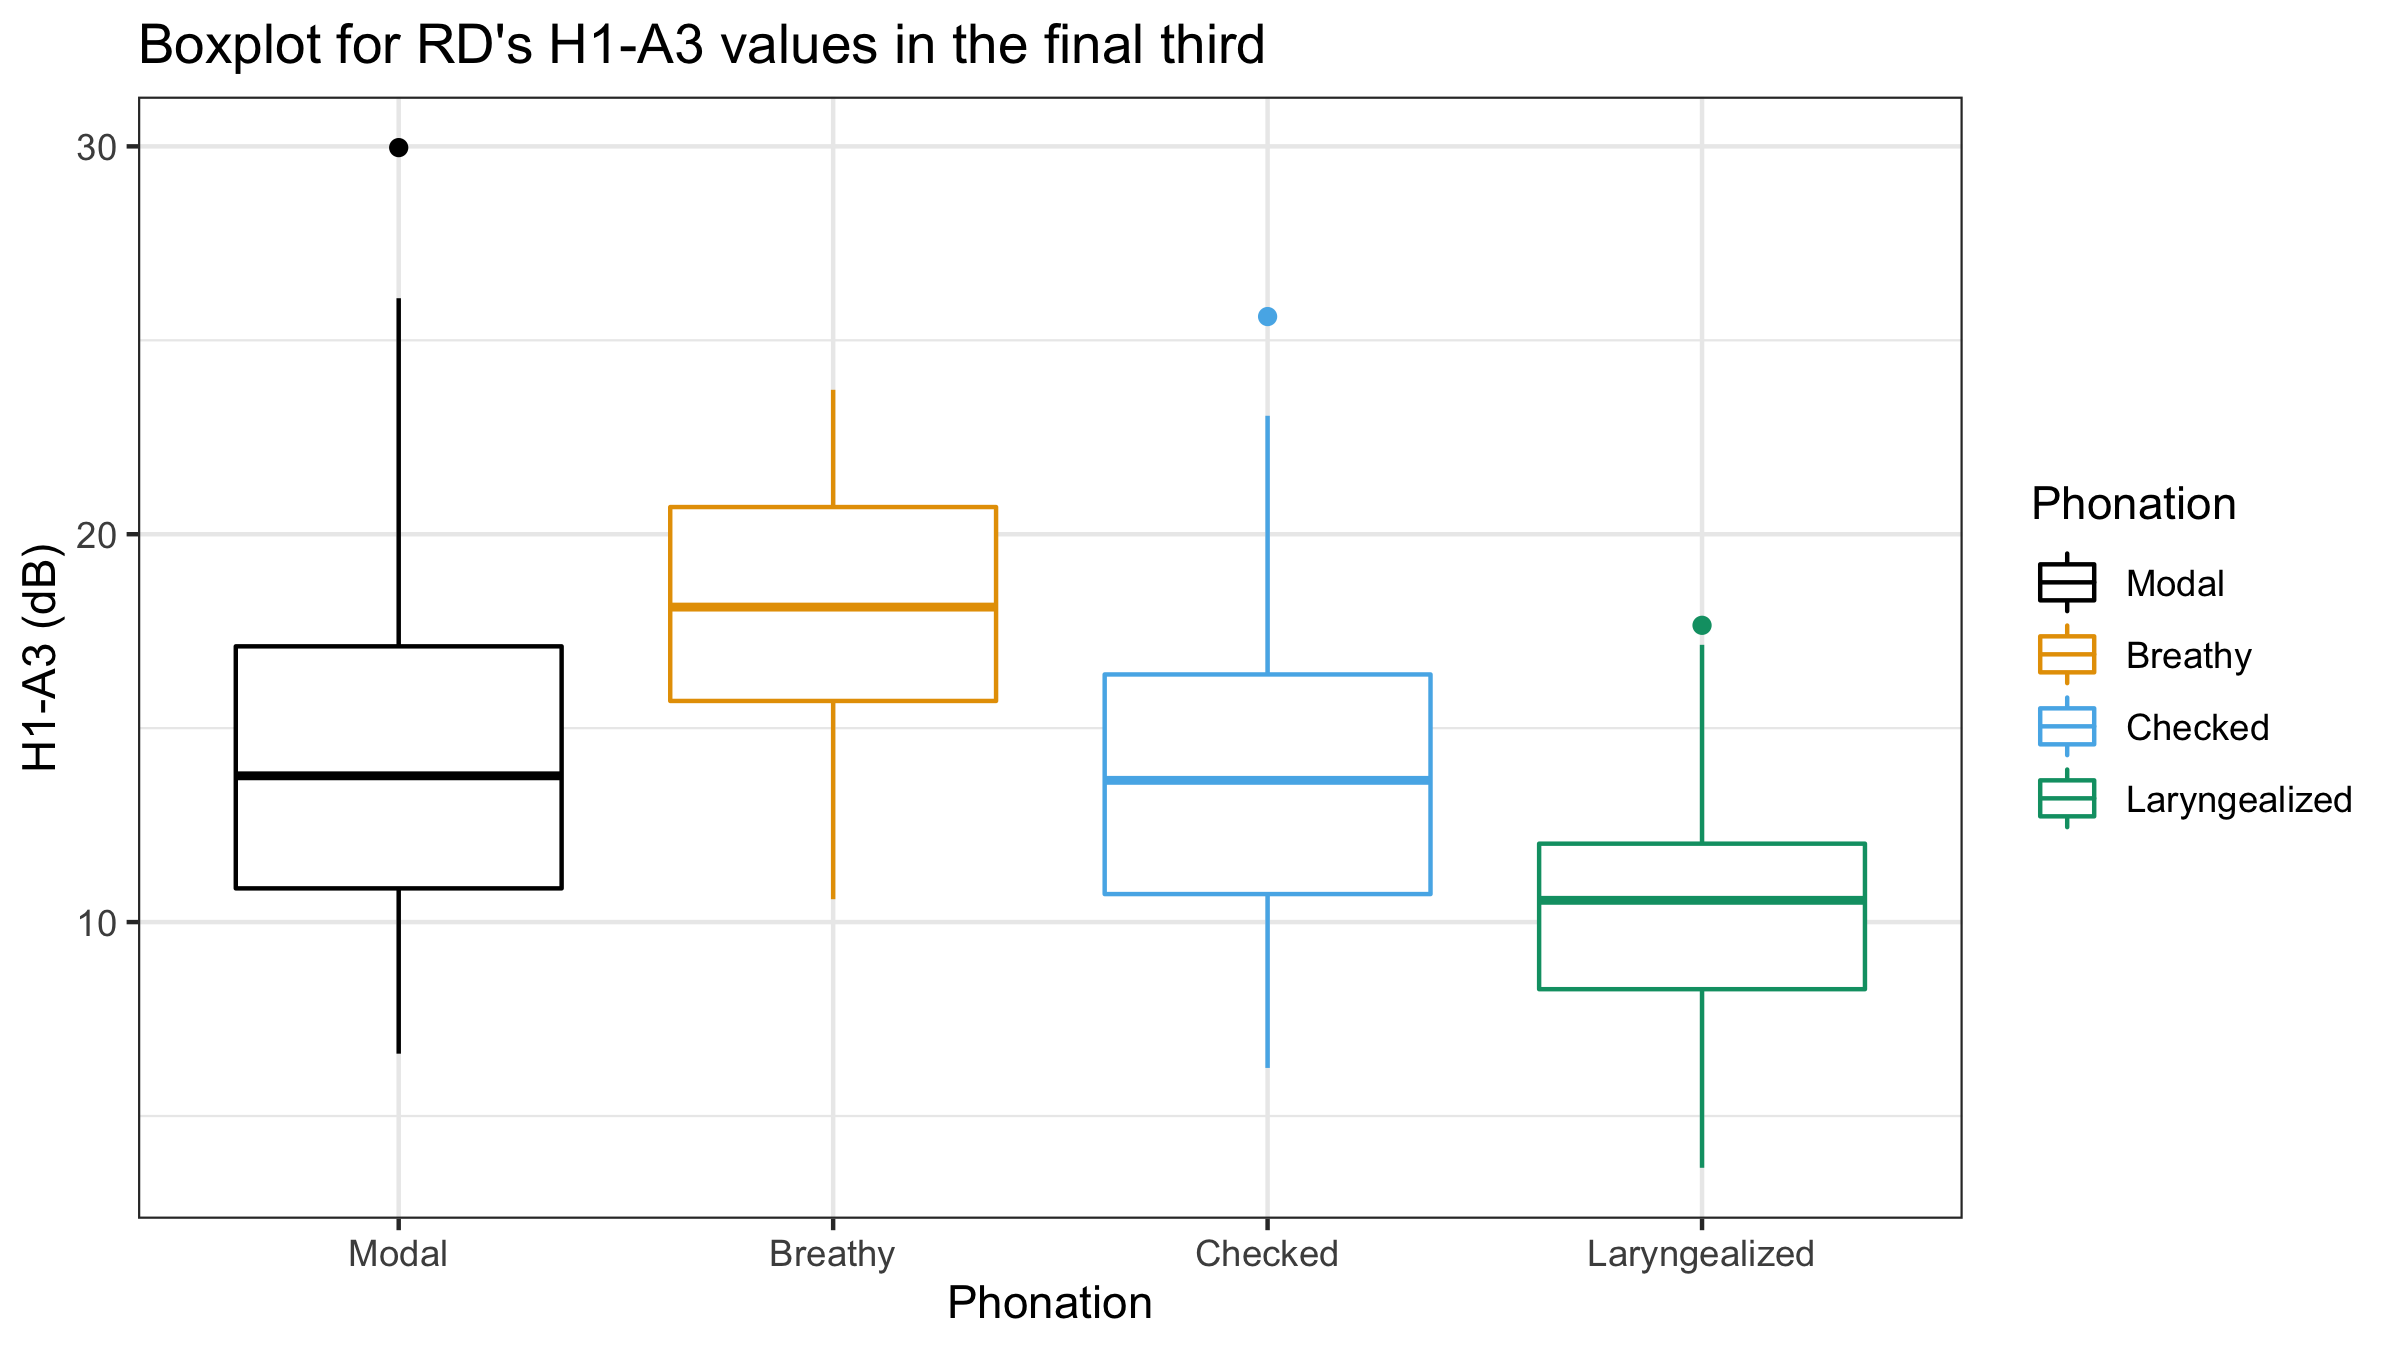
\includegraphics[width=0.9\textwidth]{../mean_RD_h1a3_third.png}
		\caption{RD's H1-A3 values.}
		\label{fig:RDh1a3third} 
	\end{subfigure}
	\caption{H1-A3 values for FSR (a) and RD (b) for the final third of the vowel. }
	\label{fig:h1a3third}
\end{figure}

\newpage
\begin{center}
	\textbf{COVID Impact}
\end{center}
\thispagestyle{empty}
Due to COVID, the pueblo of Santiago Laxopa closed itself to the outside world until a few months ago. Fortunately, I was able to elicit preliminary data from two SLZ speakers that were living in California. However, this was insufficient data to adequately assess the interaction between tone and phonation, but provided me with some preliminary results, which were presented in this abstract. I am currently, at the time of submitting this abstract, in Santiago Laxopa finishing eliciting data from additional SLZ speakers (6 male; 10 female) to verify the validity of the results of the two SLZ speakers form California. 

% \printbibliography[heading=bibintoc]

\end{document} 